\documentclass{article}
\typeout{}

\bibliographystyle{plain}
\usepackage{pythontex}
\usepackage{gensymb}
\usepackage{amssymb}
\usepackage{pgfkeys}
\usepackage{etoolbox}
\usepackage{ifthen}
\usepackage{graphicx}
\usepackage{listings}
\usepackage{xcolor}
\usepackage{booktabs}
\usepackage{array}
\usepackage{graphicx}
\usepackage{ upgreek }
\usepackage[utf8]{inputenc}
%Please add the following packages if necessary:
\usepackage{booktabs, multirow} % for borders and merged ranges
\usepackage{soul}% for underlines
\usepackage[table]{xcolor} % for cell colors
\usepackage{changepage,threeparttable} % for wide tables
\usepackage{array}     %centering of data in table
\newcolumntype{P}[1]{>{\centering\arraybackslash}p{#1}}  %centering of data in table


%New colors defined below
\definecolor{codegreen}{rgb}{0,0.6,0}
\definecolor{codegray}{rgb}{0.5,0.5,0.5}
\definecolor{codepurple}{rgb}{0.58,0,0.82}
\definecolor{backcolour}{rgb}{0.95,0.95,0.92}

%Code listing style named "mystyle"
\lstdefinestyle{mystyle}{
  backgroundcolor=\color{backcolour},   commentstyle=\color{codegreen},
  keywordstyle=\color{magenta},
  numberstyle=\tiny\color{codegray},
  stringstyle=\color{codepurple},
  basicstyle=\ttfamily\footnotesize,
  breakatwhitespace=false,         
  breaklines=true,                 
  captionpos=b,                    
  keepspaces=true,                 
  numbers=left,                    
  numbersep=5pt,                  
  showspaces=false,                
  showstringspaces=false,
  showtabs=false,                  
  tabsize=2
}


%"mystyle" code listing set
\lstset{style=mystyle}

\begin{document}
\thebibliography{mybibliography.bib}
\begin{center}
\rule{\textwidth}{1.6pt}\vspace*{-\baselineskip}\vspace*{2pt} % Thick horizontal line
\rule{\textwidth}{0.4pt}\\[\baselineskip] % Thin horizontal line

{\LARGE CATHODE RAY OSCILLIOSCOPE(C.R.O) }% Title

\rule{\textwidth}{0.4pt}\vspace*{-\baselineskip}\vspace{3.2pt} % Thin horizontal line
\rule{\textwidth}{1.6pt}\\[2\baselineskip] % Thick horizontal line




\textbf{\Large \\[\baselineskip] SGTB Khalsa College, University of Delhi}\\[\baselineskip]
\textbf{\Large Preetpal Singh(2020PHY1140) \\[\baselineskip] Anjali(2020PHY1164)}\\[\baselineskip] 

\vspace*{\baselineskip}
\textbf{\Large Unique Paper Code: 32221202}\\[\baselineskip] 
\vspace*{\baselineskip}
 
\textbf{\Large Paper Title: Waves and Optics Lab}\\[\baselineskip] 
\vspace*{\baselineskip}
\textbf{\Large Submitted on: June 16, 2021}\\[\baselineskip] 
\vspace*{\baselineskip}
\textbf{\Large Due On: June 17, 2021}\\[\baselineskip] 
\vspace*{\baselineskip}
\textbf{\Large File Name: 1140\_CRO/1164\_CRO}\\[\baselineskip]
\vspace*{\baselineskip}
\textbf{\Large B.Sc(H) Physics Sem II}\\[\baselineskip] 
\vspace*{\baselineskip}
\vspace*{\baselineskip}
\textbf{\Large Submitted to: Dr. SHAAN AMEER}\\[\baselineskip] 


\end{center}
\newpage

\section{\LARGE AIM}
\large
\begin{enumerate}
    \item To trace each of the voltage waveforms generated by the given circuit, and to measure frequency and amplitude on a virtual cathode-ray oscilloscope (vCRO)
    \item To measure the phase difference $(\phi)$ of the voltage waveforms generated by the given circuit
    \item To trace the Lissajous figure that is obtained corresponding to superposition of the voltage waveforms generated by the given circuit using a vCRO.
    \item To  plot  the  variation  of $(\phi)$ as  a  function  of  frequency  for  fixed  value  of R= 100Ω
\end{enumerate}
\section{\LARGE Apparatus required to perform experiment in lab}
\begin{itemize}
    \item AC Power source
    \item Oscillioscope
    \item Resistance
    \item Inductance/Capacitance
    \item Voltmeter etc.
\end{itemize}


\section{\LARGE THEORY}
\subsection{CATHODE RAY OSCILLIOSCOPE}
The cathode ray oscilloscope (C.R.O.) is one of the essential instrument in the physics laboratory to study d.c. as well as a.c. electric voltage variations in its magnitude and direction. We can visualize the exact nature of waveform of an a.c. voltage, particularly in amplifiers and oscillators.
\subsubsection{Cathode Ray Tube (C.R.T.)}
It consists of an evacuated glass envelop in which are an electron gun, two sets of deflection plates, focussing arrangement and a fluorescent screen.The screen is coated with a desired fluorescent material that will emit light when an electron beam strikes on the screen. The colour of spot at which the cathode rays impinge on the screen depends upon the phosphor coated inside the screen.
For example:
\newline
\vskip green : $\mathrm{Zn}$ silicate doped with $\mathrm{Mn}$. \\
\vskip blue : $\mathrm{ZnS}$ doped with $\mathrm{Ag}$. \\
\vskip red : Zn phosphate doped with Mn.
\begin{figure}[h]
    \centering
    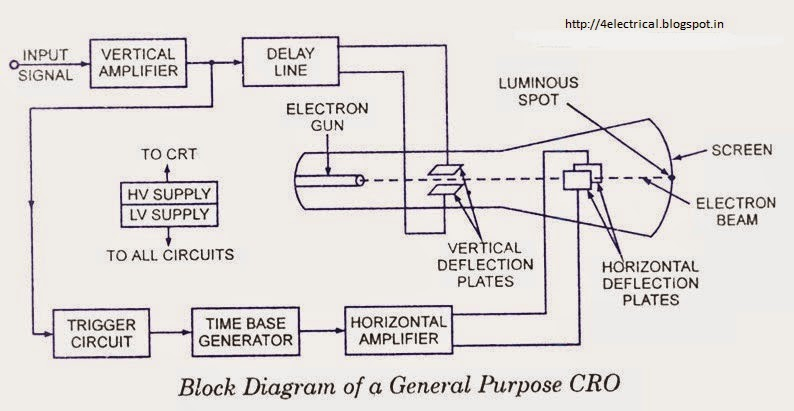
\includegraphics[width = 10cm]{CRO-Block-Diagram.jpg}
    \cite{CRO}
\end{figure}
\subsubsection{Time-base generator}
It is a saw-tooth voltage generator which provides a uniform time scale along $X$ -axis against which another voltage can be plotted by applying it to the vertical deflection plates.
\subsubsection{Synchronization}
When the frequency of sweep generator is made equal to the frequency of applied signal or some integral multiple $(n f, n=1,2,3 \ldots)$, then the sweep generator is called a synchronized sweep.
\newpage
\subsection{LISSAJOUS FIGURES}
When a particle is acted upon simultaneously by two simple harmonic motions at right angles to each other, the resultant path traced out by the particle is called the Lissajous' figure. Let the vibrations are of equal frequencies and are along $X$ and $Y$ axes, such that
$$
x=a \sin \omega t $\text { and }$$ y=b \sin (\omega t+\theta)
$$
The resultant will be given by
$$
\frac{y}{b}=\sin \omega t \cos \theta+\cos \omega t \sin \theta
$$
$$
\begin{array}{l}
=\frac{x}{a} \cos \theta+\sqrt{1-\frac{x^{2}}{a^{2}}} \sin \theta\\
\text { or }\\
\frac{x^{2}}{a^{2}}+\frac{y^{2}}{b^{2}}-\frac{2 x y}{a b} \cos \theta-\sin ^{2} \theta=0
\end{array}
$$
For, \newline
$\theta=0, \quad$ The resultant will be double straight line in the $\mathrm{I}$ and III quadrants. \\
\newline
$\theta=\pi / 4, \quad$ The resultant will be oblique ellipse with major axis in $\mathrm{I}$ and III quadrants. $\theta=\pi / 2, \quad$ The resultant will be symmetrical ellipse (or circle for $a=b$ ) \\
\newline
$\theta=3 \pi / 4$, The resultant will be oblique ellipse with major axis in II and IV quadrants.
\newpage
\subsection{LR SERIES AC CIRCUIT}
In an A.C. circuit containing $L$ and $R$ in series, the voltage across the inductor $\left(V_{L}\right)$ leads the voltage across the resistor $\left(V_{R}\right)$ by a phase angle $\pi / 2$ i.e. $90^{\circ}$ so that the resultant voltage across $L_{R}$ combination i.e. $V_{L R}$ leads the voltage (or the current $I$ across $R$ by a phase angle $\phi$ given by
$\tan \phi=\frac{L w}{R}$ where $L w=X_{L}=$ reactance due to inductance and $w=2 \pi f$ where $f$ is the frequency of
A.C. 

\begin{figure}[h]
    \centering
    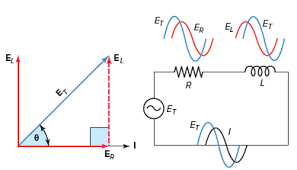
\includegraphics[width = 10cm \textwidth]{LR.png}
    \caption{R-L Circuit \citep{rl_circuit}}
    
\end{figure}

\newline

\section{\LARGE PROCEDURE}
\subsection{Procedure for vCRO}
\begin{enumerate}
\item Place the components
\begin{itemize}
\item Tap the Source subpalette and tap AC Voltage and tap on the workspace.
\item Place a resistor and inductor by dragging from the Passive subpalette.
\item Place a ground connector by dragging from the Schematic Connectors subpalette.
\item Place Voltmeter and its reference probes.
\end{itemize}
\newpage
\item Streaming data to Oscillioscope
\begin{itemize}
\item Click either through 
\includegraphics[width = 1cm, height = 1cm]{stream.png} the access command or the button on the top right.
\item Select voltage probes and click OK
\end{itemize}
\item To measure phase shift
\begin{itemize}
\item Use cursors to read specific datapoints on a graph. Drag cursors from their handles (C1, C2), or anywhere along the cursor. 
\item Measure $T_d$ by adjusting C1 and C2.
\item Note down $T_p$
\item $
\theta=T_{d} / T_{p} \times 360=10 n s / 100 n s \times 360^{\circ} \times \pi/180 =\theta_{rad}
$

\end{itemize}
\end{enumerate}
\begin{figure}[h]
    \centering
    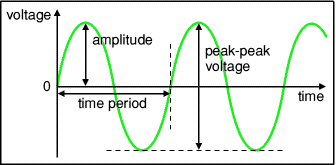
\includegraphics[width = 10cm \textwidth]{lissajous.png}
    \caption{CRO Display with Labels \cite{CRO_Display}}
\end{figure}
\newpage
\subsection{Procedure for physical Oscillioscope}
\begin{itemize}
    \item Switch 'ON' the Time/Base CRO.
    \item Connect the unknown A.C. source to $Y$ -INPUT (VER-INPUT) of the CRO.
    \item By using focus and INT knobs, obtain a sharp waveform on the screen. Now adjust TimeBase selector switch to get distinct number of waves which will be countable on the screen.
    \item The waveforms (sinusoidal, rectangular or any shape) are centered by HOR-SHIFT and VER-SHIFT knob and of proper amplitude using VER-GAIN.
    \item Set the cross wire at $k^{\text {th }}$ ring then move towards $20^{\text {th }}$ and note down the reading. 
    \item the scale count the maximum number of complete waves and the note down the distance (in $\mathrm{cm}$ ) occupying these waves. Note down the Time-Base you have selected. 
    \item Change the Time-Base and again repeat above procedure.
    
\end{itemize}

\newpage

\section{\LARGE EXPERIMENT DATA AND CALCULATIONS}
Input voltage is sinusoidal with peak-to-peak value$\left(\mathrm{V}_{p}=20 \mathrm{~V}\right)$ \\
\newline
Frequency($\omega)$ = 100Hz \\
\newline
Team Number = 29 \\
\newline
Value of Inductance, $L=$ Team no. $\times 100 \mathrm{mH}$ = 2.9$H$ \\
\newline
Resistance of inductor = 100 \Omega$ \\
\newline
Phase Difference($\theta$) = T_{d} / T_{p} \times 360 \\
\newline
\vskip =10 n s / 100 n s \times 360^{\circ} \times \pi/180 =\theta_{rad}$ \\
\newline
\vskip Here, $T_d$ and $T_p$ are time delay and time period respectively \\
\newline
x = $A_x$$\sin($2\times \omega \times t$) \\
\newline
y = $A_y$$\sin($2\times \omega \times t$ + $\theta$)
\newline
\vskip Here, $A_x$ and $A_y$ are peak amplitude of x and y waveform \\

\begin{table}[!htp] 
\centering 

\begin{tabular}{  >{\raggedright}m{1cm}  m{1.5cm}  m{1.5cm} m{1.5cm} m{1.5cm} m{1.5cm} m{5cm}  }      % centered columns (3 columns) 
\toprule                                   %inserts double horizontal lines 
R$(\Omega)$  & $A\textsubscript{x}$ $(V)$ & $A\textsubscript{y}$ $(V)$ & $T\textsubscript{d}$(ms) & $T\textsubscript{p}$(ms) & $\theta$(rad) & Lissajous Figures \\  % inserts table heading 
\midrule\addlinespace[1.5ex]
        0.1 &19.97 &1.093 &2.8125 &10 &6.08375
        & 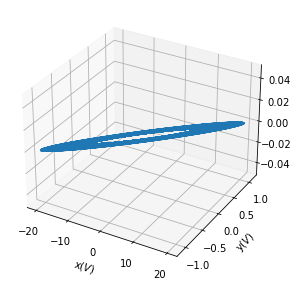
\includegraphics[height=1.5in, width=2in]{1.png} \\
\midrule\addlinespace[1.5ex]
        10 &19.97 &0.1093 &2.5 &10 &1.57 
        & 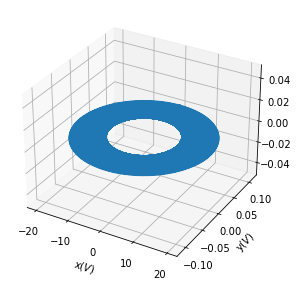
\includegraphics[height=1.5in, width=2in]{2.png} \\
\midrule\addlinespace[1.5ex]
        1K &19.97 &9.56 &1.875 &10 &1.1775
        & 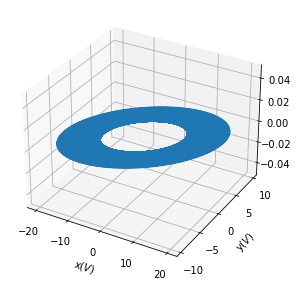
\includegraphics[height=1.5in, width=2in]{3.png} \\
\midrule\addlinespace[1.5ex]
        100K &17.005 &16.865 &0.625 &10 &0.3925
        & 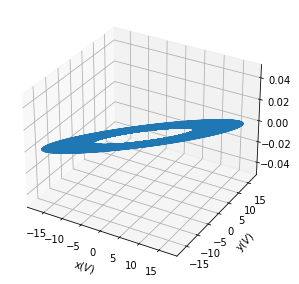
\includegraphics[height=1.5in, width=2in]{4.png} \\
\midrule\addlinespace[1.5ex]
        1M &13.54 &13.555 &0.3125 &10 &0.19625
        & 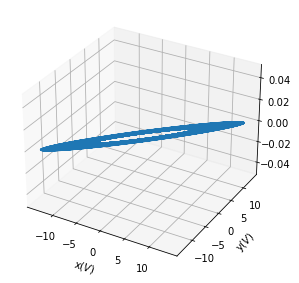
\includegraphics[height=1.5in, width=2in]{5.png} \\
\bottomrule
    \end{tabular}

    \caption{Table for Lissajous Figures with variable resistance}
    \label{table4.2}
\end{table}
\newpage
\begin{table}[!htp] 
\centering 

\begin{tabular}{  >{\raggedright}m{1cm}  m{1.5cm}  m{1.5cm} m{1.5cm} m{1.5cm} m{1.5cm} m{5cm}  }      % centered columns (3 columns) 
\toprule                                   %inserts double horizontal lines 
$v$ $(Hz)$  & $A\textsubscript{x}$ $(V)$ & $A\textsubscript{y}$ $(V)$ & $T\textsubscript{d}$(ms) & $T\textsubscript{p}$(ms) & $\theta$(rad) & Lissajous Figures \\  % inserts table heading 
\midrule\addlinespace[1.5ex]
        10 &19.97 &9.33 &15.625 &100 &0.98125
        & 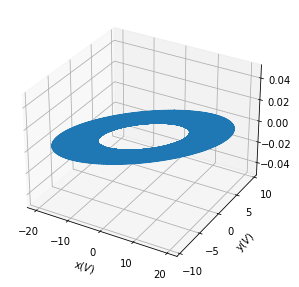
\includegraphics[height=1.5in, width=2in]{6.png} \\
\midrule\addlinespace[1.5ex]
        1K &19.97 &0.1093 &0.25 &1 &1.57 
        & 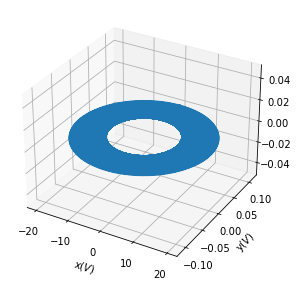
\includegraphics[height=1.5in, width=2in]{7.png} \\
\midrule\addlinespace[1.5ex]
        100K &19.97 &0.0010925 &0.0025 &0.01 &1.57
        & 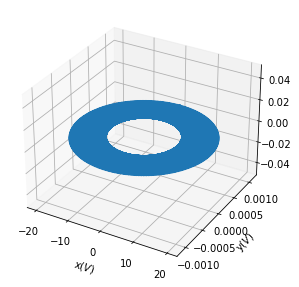
\includegraphics[height=1.5in, width=2in]{8.png} \\

\bottomrule
    \end{tabular}

    \caption{Table to form Lissajous Figures with variable Frequency}
    \label{table4.2}
\end{table}
\newpage
\section{Plotting variation  of $(\phi)$ as  a  function  of  frequency  for  fixed  value  of R= 100Ω}
\begin{figure}[h]
    \centering
    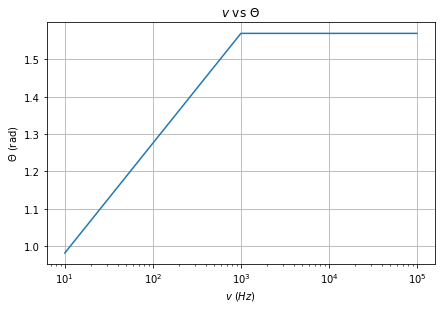
\includegraphics[width = 10cm,height = 10cm \textwidth]{v_vs_theta.png}
   
\end{figure}

\section{Discussion of Result}
\begin{itemize}
    \item We measure time delay and thus the phase difference.
    \item We plotted Lissajaus's Figures accordingly.
    \item We went through the theory of experiment by sharing links with info of concerned points and definitions.
    \item We worked together on simulator by sharing screen via GMeet.
    \item At last we jotted down the final results in a single PDF.
\end{itemize}
\section{Programming Code}
\begin{lstlisting}[language=Python]
import numpy as np
import matplotlib.pyplot as plt
import pandas as pd

def res_var():
    data = pd.read_csv('var_res.csv')
    A_x = data['Ax(in V )']
    A_y = data['Ay(in V )']
    delta = data['delta( in rad)']
    t = np.linspace(-np.pi,np.pi,300)

    for i in range(0,5):
        x = A_x[i]*np.sin(2*100* t)
        y = A_y[i]*np.sin(2*100* t + delta[i])
        fig = plt.figure()
        ax = plt.axes(projection='3d')
        ax.set_xlabel("x($V$)")
        ax.set_ylabel("y($V$)")
        plt.tight_layout()
        ax.grid(True)
        plt.plot(x,y)
        plt.show()
        
def freq_var():
    data = pd.read_csv('var_freq.csv')
    A_x = data['Ax(in V )']
    A_y = data['Ay(in V )']
    delta = data['delta( in rad)']
    t = np.linspace(-np.pi,np.pi,300)

    for i in range(0,3):
        x = A_x[i]*np.sin(2*100* t)
        y = A_y[i]*np.sin(2*100* t + delta[i])
        fig = plt.figure()
        ax = plt.axes(projection='3d')
        ax.set_xlabel("x($V$)")
        ax.set_ylabel("y($V$)")
        plt.tight_layout()
        ax.grid(True)
        plt.plot(x,y)
        plt.show()
        
def delta_vs_freq():
    data = pd.read_csv('var_freq.csv')
    delta = data['delta( in rad)']
    freq = data['v(Hz)']
    
    plt.xscale('log')
    plt.tight_layout()
    plt.grid(True)
    plt.xlabel("$v$ $(Hz)$")
    plt.ylabel("$\Theta$ (rad)")
    plt.title("$\Theta$ vs $v$")
    plt.plot(freq,delta)
    plt.show()
    
def freq_not():
    data = pd.read_csv('var_freq.csv')
    v = data['v(Hz)']
    Ax = data['Ax(in V )']
    Ay = data['Ay(in V )']
    fig, ax = plt.subplots()
    ax.plot(v,Ax)
    ax.plot(v,Ay)
    ax.set_xlabel("$A_x(V)$")
    ax.set_ylabel("$A_y(V)$")
    plt.xticks(np.arange(12, 21, 1.0))
    plt.yticks(np.arange(0, 18, 2.5))
    #ax.annotate("(17,17)", (17,17),xytext=(17,17))
    plt.title("$A_x$ vs $A_y$")
    plt.grid(True)
    plt.show()
    

        
if __name__ == "__main__":
    res_var()
    freq_var()
    delta_vs_freq()
    

\end{lstlisting}
\section{Precautions}
\begin{itemize}
    \item The Time-Base must be selected properly.
    \item The pattem must be steady. Hence locking must be done by SYNC. control.
    \item The beginning of first wave should start from extreme left of the scale.
    \item Note down carefully the distance $L$ on $X$ -axis that occupies $n$ waves.
    \item For more accuracy, take maximum number of waves on the screen (of course complete waves).
\end{itemize}

\section{RESULT}
{\Large Lissajous Figures formed successfully.


\end{frame}

\section{Contribution of each Partner}
{\Bold Partner A} \\
Name: Anjali \\
Roll No. : 2020PHY1164 \\
Contributions : \\
\begin{enumerate}
    \item Theory
    \item Procedure
    \item Experiment Data and Calculations
    \item Error Correction
\end{enumerate}
\newline
{\Bold Partner B} \\
Name: Preetpal Singh \\
Roll No. : 2020PHY1140 \\
Contributions : \\
\begin{enumerate}
    \item Theory
    \item Procedure
    \item Experiment Data and Calculations
    \item Programming Code
\end{enumerate}
\section{REFERENCES}
\cite{harnam}
\cite{CRO_Display}
\cite{CRO}
\cite{rl_circuit}

\end{document}
